\documentclass[aspectratio=169]{beamer}

\usetheme{Boadilla}

\usepackage[english]{babel}
\usepackage[latin1]{inputenc}
\usepackage{times}
\usepackage[T1]{fontenc}
\usepackage{amsmath}
% \usepackage{psfrag}
\usepackage{graphics}
\usepackage{color}
\usepackage{cancel}
\usepackage{listings}
%\usepackage{movie15}
\usepackage{multimedia}
% \usepackage{epstopdf}
% \usepackage{caption}
\usepackage{graphicx}
%\usepackage{subcaption}
\usepackage{comment}
\usepackage{colortbl}
\usepackage[absolute,overlay]{textpos}

\newcommand{\backupbegin}{
    \newcounter{finalframe}
    \setcounter{finalframe}{\value{framenumber}}
}
\newcommand{\backupend}{
    \setcounter{framenumber}{\value{finalframe}}
}
\lstset{language=[90]Fortran,
    basicstyle=\ttfamily\scriptsize,
    keywordstyle=\color{red},
    commentstyle=\color{blue},
    morecomment=[l]{!\ }% Comment only with space after !
}

\newcommand{\ol}[1]{\overline{#1}}
\newcommand{\olu}{\overline{u}}
\newcommand{\olp}{\overline{p}}
\newcommand{\olv}{\overline{v}}
\newcommand{\ot}[1]{\widetilde{#1}}
\newcommand{\otu}{\widetilde{u}}
\newcommand{\otp}{\widetilde{p}}
\newcommand{\otv}{\widetilde{v}}
\newcommand{\otw}{\widetilde{w}}
\newcommand{\hx}{\hat{x}}
\newcommand{\hatt}{\hat{t}}

\newcommand{\myworry}[1]{\textcolor{red}{#1}} % MK added
\newcommand{\karman}{von K\'{a}rm\'{a}n } % MK added
\newcommand{\intd}{\;\textrm{d}} % MK added
\newcommand{\pdiff}[2]{\frac{\partial #1}{\partial #2}}
%\newcommand\Rey{\mbox{\textit{Re}}}  % Reynolds number
\newcommand{\yp}{$y^+$ }
\newcommand{\uu}{$\langle u'^2 \rangle$ }
\newcommand{\vv}{$\langle v'^2 \rangle$ }
\newcommand{\ww}{$\langle w'^2 \rangle$ }
\newcommand{\uv}{$\langle u'v' \rangle$ }
\newcommand{\uw}{$\langle u'w' \rangle$ }
\newcommand{\vw}{$\langle v'w' \rangle$ }
\newcommand{\uup}{$\langle u'^2 \rangle^+$ }
\newcommand{\vvp}{$\langle v'^2 \rangle^+$ }
\newcommand{\wwp}{$\langle w'^2 \rangle^+$ }
\newcommand{\uvp}{$\langle u'v' \rangle^+$ }
\newcommand{\uwp}{$\langle u'w' \rangle^+$ }
\newcommand{\vwp}{$\langle v'w' \rangle^+$ }
\newcommand{\REF}{\textrm{ref}}
\newcommand{\D}{\mathrm{d}}

\def\LS#1{#1_{\textrm{LS}}}
\def\SS#1{#1_{\textrm{SS}}}
\def\bk{\mathbf{k}}
\def\uupss{ $\langle u'^2 \rangle^+_{\textrm{SS}}$ }
\def\vvpss{ $\langle v'^2 \rangle^+_{\textrm{SS}}$ }
\def\wwpss{ $\langle w'^2 \rangle^+_{\textrm{SS}}$ }
\def\uupls{ $\langle u'^2 \rangle^+_{\textrm{LS}}$ }
\def\vvpls{ $\langle v'^2 \rangle^+_{\textrm{LS}}$ }
\def\wwpls{ $\langle w'^2 \rangle^+_{\textrm{LS}}$ }
\title[Batch Random Optimizer]{A Batch-Random Algorithm for Learning on Distributed, Heterogeneous Data}
\author[P. Mohan]{Prakash Mohan, Marc Henry de Frahan, Ryan King, Ray Grout}
% \institute[U of Texas, Austin]%{University of Texas at Austin\\}
% {
%     Institute for Computational Engineering and Sciences \\
%     University of Texas at Austin
% }
\date[October 2018]{\small October 2018}
\setbeamertemplate{navigation symbols}{}
\begin{document}

\begin{frame}
    \titlepage
\end{frame}

% ---------------------------------------------------------------------------------------------------------------------------------
\begin{frame}
    \frametitle{Exascale Computations}
    \begin{itemize}
        \item Simulating complex physics problems is computationally expensive
        \item Example: Turbulent channel flow
            \begin{itemize}
                \item Direct numerical simulation at $Re_{\tau} = 5200$ had $696 \times 10^9$ degrees of freedom
                \item Took $\sim400$ million core hours to finish
                \item Practical flows are at $Re_{\tau} = 10^5$ or even $10^6$
            \end{itemize}
        % \item Can we effectively utilize data from expensive computations?
        \item Leverage high fidelity simulations to develop reduced order models
        \item Machine learning has shown to be effective in building accurate models from data
    \end{itemize}
\end{frame}
%---------------------------------------------------------------------------------------------------------------------------------
\begin{frame}
    \frametitle{Machine Learning Performance}
    \begin{figure}
        \centering
        \includegraphics[width=0.65\textwidth]{figs/data_size_vs_model_performance}
    \end{figure}
\end{frame}
% ---------------------------------------------------------------------------------------------------------------------------------
 \begin{frame}
     \frametitle{Deep Neural Networks (DNNs)}
     \begin{itemize}
         \item Set of algorithms, loosely designed after the human brain to learn features
         \item More effective than other traditional forms of machine learning
         \item Can learn quickly on large data and are very performant given the nature of computations involved
         \item Widely used in everyday applications: image recognition, speech transcription
         \item Bigger applications: self-driving cars, alpha-go
         \item Increase in computing power and data available makes them very successful
         \item Can incrementally learn as more data becomes available
     \end{itemize}
 \end{frame}
%---------------------------------------------------------------------------------------------------------------------------------
\begin{frame}
    \frametitle{How do DNNs work?}
    \begin{figure}
        \centering
        \includegraphics[width=0.65\textwidth]{figs/dnn_schematic}
    \end{figure}
\end{frame}
%---------------------------------------------------------------------------------------------------------------------------------
\begin{frame}
    \frametitle{How do DNNs work?}
    \begin{figure}
        \centering
        \includegraphics[width=0.6\textwidth]{figs/dnn_flow}
    \end{figure}
\end{frame}
%---------------------------------------------------------------------------------------------------------------------------------
\begin{frame}
    \frametitle{How do DNNs work?}
    \begin{figure}
        \centering
        \includegraphics[width=0.75\textwidth]{figs/dnn_weights}
    \end{figure}
\end{frame}
%---------------------------------------------------------------------------------------------------------------------------------
\begin{frame}
    \frametitle{Learning parameters in the DNN}
    \begin{itemize}
        \item Define a cost function to compare outputs to data
        \item Compute the gradient of this cost function, and move in the opposite direction
        \item Deterministic gradient descent is slow when dealing with large amounts of data
        \item Variants of mini-batch gradient descent are typically used for deep learning
        \item These algorithms rely on data being randomly shuffled to avoid bias across batches
    \end{itemize}
\end{frame}
% ---------------------------------------------------------------------------------------------------------------------------------
\begin{frame}
    \frametitle{Online Learning on Exascale Computations}
    \begin{itemize}
        \item As simulations grow larger, storing high-fidelity data is also expensive (disk I/O, storage costs)
        \item Need to train models with the computations, minimizing disk I/O
        \item The shuffling operation for mini-batch gradient descent is infeasible online
        \item Simulations tend to be spatially heterogeneous, batches from any given node will have high bias
        \item Algorithms that sequentially train across batches will fail in this setting
    \end{itemize}
\end{frame}
%---------------------------------------------------------------------------------------------------------------------------------
\begin{frame}
  \frametitle{Streamwise velocity \& wall-shear stress in a channel flow}
  \vspace{6pt}
  \begin{figure}
    \centering
    \reflectbox{\includegraphics[width=.85\textwidth]{figs/5200_u_XY_u_YZ_omega_z_XZ}}
  \end{figure}
  \vspace{6pt}
\end{frame}
%---------------------------------------------------------------------------------------------------------------------------------
\begin{frame}
    \frametitle{Proposed algorithm: Batch-Randomized Gradient Descent}
    \begin{itemize}
        \item Instead of training sequentially across batches, pick batches in a random order
        \item Useful in cases where the data has some ordering and shuffling is not an option
        \item Ideal for distributed problems, pick nodes at random to get batches from
        \item Avoids feeding data with the same bias into the optimizer multiple times in a row
    \end{itemize}
\end{frame}
%---------------------------------------------------------------------------------------------------------------------------------
\begin{frame}
    \frametitle{Benchmarks on classification problems}
    \begin{itemize}
        \item Use standardized datasets for benchmarking on classification problems
        \item Three different scenarios:
            \begin{itemize}
                \item Fully shuffled data with mini-batch gradient descent
                \item Data sorted by classes with mini-batch gradient descent
                \item Data sorted by classes with batch-random gradient descent
            \end{itemize}
        \item Data being sorted this way is a proxy for spatial heterogeneity in physics based problems
    \end{itemize}
\end{frame}
%---------------------------------------------------------------------------------------------------------------------------------
\begin{frame}
    \frametitle{Benchmarks on classification problems}
    \begin{figure}
        \centering
        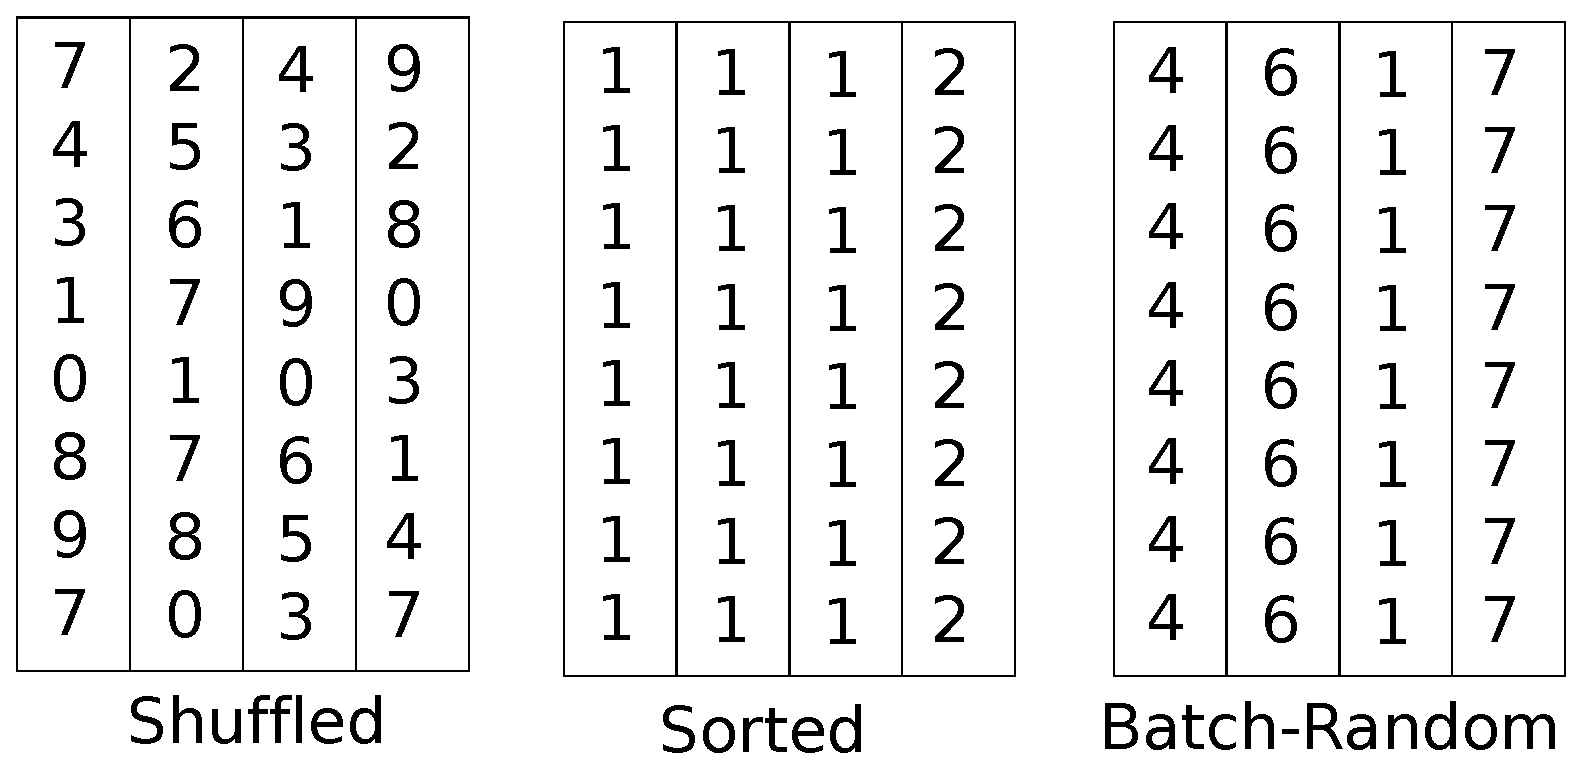
\includegraphics[width=0.8\textwidth]{figs/batch-random}
    \end{figure}
\end{frame}
%---------------------------------------------------------------------------------------------------------------------------------
\begin{frame}
    \frametitle{Benchmark 1: MNIST dataset, 10 classes, 70000 samples}
    \begin{figure}
        \centering
        \includegraphics[width=0.65\textwidth]{figs/mnist_samples}
    \end{figure}
\end{frame}
%---------------------------------------------------------------------------------------------------------------------------------
\begin{frame}
    \frametitle{Benchmark 1: MNIST dataset, 10 classes, 70000 samples}
    \begin{figure}
        \centering
        \includegraphics[width=0.65\textwidth]{figs/mnist}
    \end{figure}
\end{frame}
%---------------------------------------------------------------------------------------------------------------------------------
\begin{frame}
    \frametitle{Benchmark 2: Digits dataset, 10 classes, 280000 samples}
    \begin{figure}
        \centering
        \includegraphics[width=0.65\textwidth]{figs/digits}
    \end{figure}
\end{frame}
%---------------------------------------------------------------------------------------------------------------------------------
\begin{frame}
    \frametitle{Benchmark 3: Fashion dataset, 10 classes (hard), 70000 samples}
    \begin{figure}
        \centering
        \includegraphics[width=0.5\textwidth]{figs/fashion_samples}
    \end{figure}
\end{frame}
%---------------------------------------------------------------------------------------------------------------------------------
\begin{frame}
    \frametitle{Benchmark 3: Fashion dataset, 10 classes (hard), 70000 samples}
    \begin{figure}
        \centering
        \includegraphics[width=0.65\textwidth]{figs/fashion}
    \end{figure}
\end{frame}
%---------------------------------------------------------------------------------------------------------------------------------
\begin{frame}
    \frametitle{Benchmark 4: Letters dataset, 26 classes, 145600 samples}
    \begin{figure}
        \centering
        \includegraphics[width=0.5\textwidth]{figs/letters_samples}
    \end{figure}
\end{frame}
%---------------------------------------------------------------------------------------------------------------------------------
\begin{frame}
    \frametitle{Benchmark 4: Letters dataset, 26 classes, 145600 samples}
    \begin{figure}
        \centering
        \includegraphics[width=0.65\textwidth]{figs/letters}
    \end{figure}
\end{frame}
%---------------------------------------------------------------------------------------------------------------------------------
\begin{frame}
    \frametitle{Benchmark 5: Combined dataset, 62 classes, 814255 samples}
    \begin{figure}
        \centering
        \includegraphics[width=0.65\textwidth]{figs/byclass}
    \end{figure}
\end{frame}
%---------------------------------------------------------------------------------------------------------------------------------
\begin{frame}
    \frametitle{Dependence on Batch Size}
    \begin{figure}
        \centering
        \includegraphics[width=0.65\textwidth]{figs/block_size_to_bin_count-log}
    \end{figure}
\end{frame}
%---------------------------------------------------------------------------------------------------------------------------------
\begin{frame}
    \frametitle{Turbulent Channel flow}
  \vspace{6pt}
  \begin{figure}
    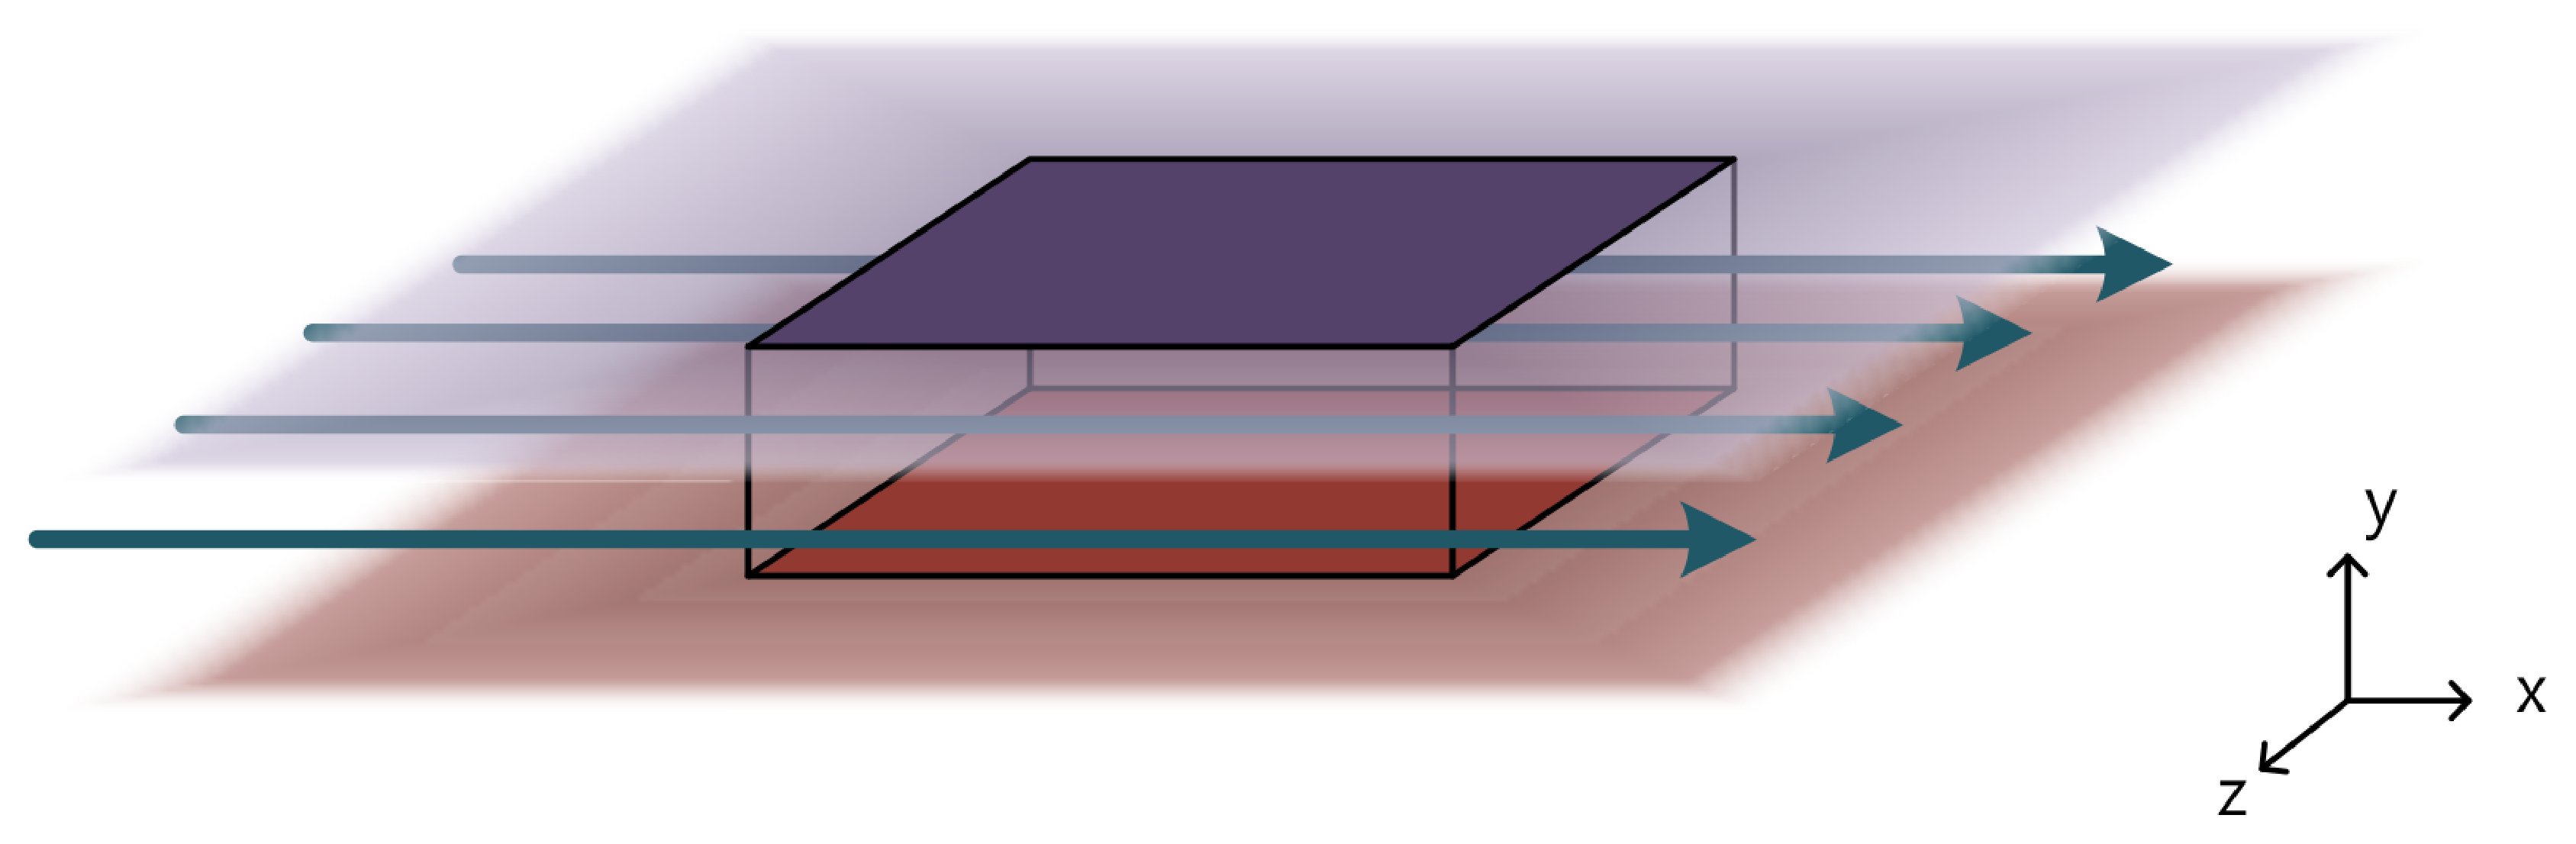
\includegraphics[width=0.7\textwidth]{figs/simulation_geometry}
  \end{figure}
  \begin{itemize}
  \item Flow between infinite parallel planes
  \end{itemize}
  \vspace{6pt}
\end{frame}
%---------------------------------------------------------------------------------------------------------------------------------
\begin{frame}
    \frametitle{Large Eddy Simulations (LES)}
    \begin{itemize}
        \item Objective is to perform predictive simulations of high-Re flows
        \item DNS is too expensive, and cost scales roughly as $Re^{\frac{11}{4}}$
        \item The main idea behind LES is to only simulate ``large'' scales of turbulence
        \item It is reasonable to expect the small scale motions to be universal, so easier to model those
        \item Define a filter, apply it on the governing equations and simulate the filtered system
    \end{itemize}
\end{frame}
%---------------------------------------------------------------------------------------------------------------------------------
\begin{frame}
    \frametitle{Closure problem in LES}
    Governing equations for LES, filter represented by $\ot{\cdot}$
    \begin{align}
    \frac{\partial \otu^+_i}{\partial t^+}+\frac{\partial \otu^+_i\ot u^+_j}{\partial
      x^+_j}&=-\frac{\partial \otp^+}{\partial x^+_i}+\frac{\partial^2 \otu^+_i}{\partial
      x^+_j\partial x^+_j}+\frac{\partial \tau_{ij}}{\partial x^+_j}\\
    \frac{\partial \ot u^+_i}{\partial x^+_i}&=0
\end{align}
where,
\begin{equation}
\tau_{ij}=-\ot{u^+_iu^+_j}+\otu^+_i\otu^+_j.
\end{equation}
Can we predict $\tau$ using pointwise velocities and gradients?
\end{frame}
%---------------------------------------------------------------------------------------------------------------------------------
\begin{frame}
    \frametitle{Large Eddy Simulations (LES)}
    \begin{figure}
        \centering
        \includegraphics[width=0.6\textwidth]{figs/les}
    \end{figure}
\end{frame}
%---------------------------------------------------------------------------------------------------------------------------------
\begin{frame}
    \frametitle{2D energy spectra of \uu at $y^+ = 15$ \footnote{\scriptsize Lee and Moser, ``Spectral analysis of the budget equation in turbulent channel flows at high $Re$''}}
    \begin{columns}[c]
        \column{0.45\textwidth}
        \includegraphics[width=\textwidth]{figs/2d_uu_y_plus_15}
        \column{0.55\textwidth}
        \begin{itemize}
            \item Universal small scale behavior
            \item Small scale peak smeared by outer flow
            \item Outer-flow dependent large scales
            \item Indicates a horizontal filter width $\Delta^+\approx 1500$
        \end{itemize}
    \end{columns}
\end{frame}
%---------------------------------------------------------------------------------------------------------------------------------
\begin{frame}
    \frametitle{High-pass / low-pass filtered statistics of velocity variances \footnote{\scriptsize Lee and Moser, ``Spectral analysis of the budget equation in turbulent channel flows at high $Re$''}}
    \begin{figure}
        \centering
        \includegraphics[width=0.5\textwidth]{figs/Filtering_uu}
    \end{figure}
\end{frame}
%---------------------------------------------------------------------------------------------------------------------------------
%---------------------------------------------------------------------------------------------------------------------------------
\begin{frame}
    \frametitle{WALE model for $\tau_{ij}$}
    \begin{figure}
        \centering
        \includegraphics[width=0.65\textwidth]{figs/WALE}
    \end{figure}
\end{frame}
%---------------------------------------------------------------------------------------------------------------------------------
\begin{frame}
    \frametitle{Random Forest predictions for $\tau_{ij}$}
    \begin{figure}
        \centering
        \includegraphics[width=0.65\textwidth]{figs/pred_uv_rf}
    \end{figure}
\end{frame}
%---------------------------------------------------------------------------------------------------------------------------------
\begin{frame}
    \frametitle{Random Forest predictions for $\tau_{ij}$}
    \begin{figure}
        \centering
        \includegraphics[width=0.65\textwidth]{figs/pred_uv_rf-hist}
    \end{figure}
\end{frame}
%---------------------------------------------------------------------------------------------------------------------------------
\begin{frame}
    \frametitle{Feed-Forward DNN predictions for $\tau_{ij}$ (4 hidden layers with 10 nodes)}
    \begin{figure}
        \centering
        \includegraphics[width=0.65\textwidth]{figs/pred_uv_dnn}
    \end{figure}
\end{frame}
% ---------------------------------------------------------------------------------------------------------------------------------
\begin{frame}
    \frametitle{Feed-Forward DNN predictions for $\tau_{ij}$ (4 hidden layers with 10 nodes)}
    \begin{figure}
        \centering
        \includegraphics[width=0.65\textwidth]{figs/pred_uv_dnn-hist}
    \end{figure}
\end{frame}
% ---------------------------------------------------------------------------------------------------------------------------------
 \begin{frame}
     \frametitle{Summary and path forward}
         \begin{itemize}
             \item Batch-random optimizer is effective for training on distributed, heterogeneous data
             \item DNNs are very good at predicting on classification problems
             \item Lots of room for progress in predicting $\tau_{ij}$
             \item Perhaps a rethinking of DNNs for regression is warranted
             % \item Perform LES with the model from RF or DNN to check {\it aposteriori} performance
         \end{itemize}
 \end{frame}
% ---------------------------------------------------------------------------------------------------------------------------------
\begin{frame}
    \begin{center}
        \vspace{6pt}
        {\huge Thank you!} \\
        \vspace{12pt}
        {\huge Questions?}
    \end{center}
\end{frame}
%---------------------------------------------------------------------------------------------------------------------------------
\backupbegin
\backupend
\end{document}
